% !TeX root = ../main.tex

\chapter{医学文本生成任务训练阶段的隐私保护研究}

\section{引言}

%为防止攻击者在训练阶段试图推断隐私数据以及破坏训练协议的攻击,本章提出了一个基于秘密共享\cite{SecretSharingAS, Shamir_SS}的安全训练协议。

%本章主要研究医学文本生成任务训练阶段中的隐私保护问题,旨在提供一种可以抵抗恶意攻击者的安全协议,以保护医学文本数据在训练阶段的隐私。首先,本章明确了模型与设计目标,在阐述了系统模型与威胁模型的基础上提出了安全目标。然后,本章扩展了基于加法秘密共享的协议,使其能够支持复杂的Transformer结构,通过这种方式来保护数据的机密性。此外,本章还通过Intel SGX来保障过程的完整性,并针对可并行计算的矩阵乘法部分设计了一个外包计算协议来提高执行效率。接着,本章分析了协议的安全性,证明了它能够满足设计目标。最后,本章通过实验证明了协议的有效性和高效性。

本章主要针对医学文本生成任务训练阶段的隐私问题,设计并实现一种能够有效抵抗恶意攻击者的安全协议。首先,本章明确了模型与设计目标,在阐述了系统模型与威胁模型的基础上提出了安全目标。随后,为保护数据的机密性,本章扩展了基于加法秘密共享的协议,使其能够适配Transformer的复杂结构。此外,为确保执行过程的完整性,本章引入SGX,同时为提高计算效率,针对可并行计算的矩阵乘法部分,本章设计了一个高效的外包计算协议。随后,本章进行了协议安全性的分析,并通过理论证明验证其能满足设计目标。最后,本章通过实验证明了该协议的有效性和高效性。

%在系统模型和威胁模型的基础上,本部分设计了安全目标,并提出了基于秘密共享的多方安全计算协议以保障机密性。为确保执行过程的完整性,本章引入了可信硬件Intel SGX,还扩展了基于秘密共享的协议,使其能够支持复杂的Transformer结构,并针对可并行计算的矩阵乘法部分设计了一个外包计算协议来提高执行效率。接着,本章分析了协议的安全性,证明了它能够满足设计目标。最后,本章通过实验证明了协议的有效性和高效性。

\section{模型与设计目标} \label{chap2_system_model}

\subsection{系统模型}

%在这种场景下,我们假设有两类实体,一方是多个拥有医疗隐私数据的数据持有者,另一方是提供计算服务的多个计算方。多个数据持有者希望通过多个计算方提供的计算服务来协同训练模型,计算方在计算服务结束后将训练好的模型分发给各个数据持有者。

%在这种场景下,我们假设有两类实体,一方是多个拥有医学隐私数据的数据持有者,另一方是提供计算服务的多个计算方。多个数据持有者希望通过多个计算方提供的计算服务来协同训练模型,计算方在计算服务结束后将训练好的模型分发给各个数据持有者。本章只关注训练过程中隐私数据的安全性问题。

%如图\ref{Chap4_System_Info}所示,其中①表示多个数据持有者通过秘密共享算法将数据拆分成两个秘密份额分发给服务器$p_0$与服务器$p_1$。②表示在服务器$p_2$提供的相应MPC计算随机数的辅助下,服务器$p_0$与服务器$p_1$运行MPC协议来执行模型的训练过程。③表示训练结束后,服务器$p_0$与服务器$p_1$将各自的模型参数份额返还给各数据持有者。在这种场景下,我们假设有两类实体,一方是多个拥有医疗隐私数据的数据持有者,另一方是提供计算服务的三个计算方。多个数据持有者希望通过多个计算方提供的计算服务来协同训练模型,计算方在计算服务结束后将训练好的模型分发给各个数据持有者。其中作为提供计算服务的三个计算方$p_0$、$p_1$与$p_2$均具有Intel SGX,且$p_0$与$p_1$具有高性能计算GPU或者TPU(后文均以GPU指代)。

在这种场景下,本章假设有两类实体,一类是多个拥有医学文本数据(患者医疗隐私数据)的数据持有者,另一类是提供计算服务的三个计算方。多个数据持有者希望通过多个计算方提供的计算服务来协同训练模型,计算方在计算服务结束后将训练好的模型分发给各个数据持有者。其中作为提供计算服务的三个计算方$p_0$、$p_1$与$p_2$均具有Intel SGX,且$p_0$与$p_1$具有高性能计算GPU或者TPU(后文均以GPU指代)。如图 \ref{Chap4_System_Info} 所示,其中①表示多个数据持有者通过秘密共享机制\cite{SecretSharingAS, Shamir_SS}将数据拆分成两个秘密份额分发给服务器$p_0$与服务器$p_1$。②表示在服务器$p_2$提供的相应MPC计算随机数的辅助下,服务器$p_0$与服务器$p_1$运行MPC协议来执行模型的训练过程。③表示训练结束后,服务器$p_0$与服务器$p_1$将各自的模型参数份额返还给各数据持有者。本章只关注训练过程中隐私数据的安全性问题。

%转到医学文本生成任务这一具体场景下,由于本文是基于预训练模型在医学文本数据上进行微调的,而本文使用的预训练模型是在大量中文语料上训练的通用预训练模型,涵盖了各种通用领域的数据常见,并且医学文本场景下的数据两较少,因此为了避免在此小数据量微调时过拟合并充分利用预训练的词嵌入优势,本文后续的实验中会固定预训练的词嵌入,即\ref{generate_word_embd}节中的Word Embedding在微调过程中固定。此外,由于预训练模型的词表涵盖各种场景,医学文本领域中复用预训练的词表(词表大小为21128)也不会有UNK(即不在词表上的Token),因此,后续实验也不会根据医学文本进行重构词表。
%
%以训练医学问答模型的场景为例,假设有多个数据持有者(如医院),每个数据持有者拥有一个本地医学文本数据集,为了协同训练,每一方根据模型的词表将各自的数据集切词整理成一个Tokens数据集,并根据预训练模型的Word Embedding将其训练数据处理成完整的Embedding,并根据秘密共享机制将其查分成秘密份额,分发给计算方服务器。初始的预训练模型根据秘密共享算法查分放在两个计算方服务器上。在第三个服务器提供辅助计算的情况下,两个计算方服务器根据各自的Embedding份额一次通过模型,完成前向计算。数据持有者根据两个计算方服务器计算结果进行重构并根据己方的真值得到损失,并更新计算方服务器的参数。

在将本研究应用于医学文本生成任务的具体场景时,本章依托于预训练模型在医学文本数据上进行微调。所使用的预训练模型是基于广泛的中文语料进行训练的通用模型,包含了各种领域的常见数据。由于医学文本数据在总量上相对较小,为了避免微调过程中的过拟合问题,同时最大限度地利用预训练词嵌入的优势,本章决定在微调阶段固定预训练的词嵌入。这意味着在接下来的实验中,\ref{generate_word_embd} 节中所述的Word Embedding在微调过程中将保持不变。

此外,鉴于预训练模型的词表涵盖了各种领域,而医学文本领域的特有词汇在该词表中也可找到对应的Token,因此本章无需为医学文本重构词表,而是直接复用预训练模型的词表(词表大小为21128)。

特别地,以医学问答模型的训练场景为例,假设存在多个数据持有者(例如医院),每一方都拥有一份本地医学文本数据集。为了实现协同训练,每个数据持有者首先根据模型的词表将自己的数据集进行切词,整理成Token数据集。然后,根据预训练模型的Word Embedding将这些Token转化为完整的词嵌入。接着,通过秘密共享机制,将词嵌入拆分成秘密份额,然后分发给各计算方服务器。同时,初始预训练模型也根据秘密共享机制被拆分,并存储在两个计算方服务器上。在第三个服务器提供辅助计算的情况下,两个计算方服务器根据各自的词嵌入份额通过执行设计的计算协议进行一次模型前向计算。数据持有者接着根据两个计算方服务器的计算结果进行重构,并依据本地的真实值计算出损失,再根据此损失更新计算方服务器上的参数。

\begin{figure}[h]
	\centering
	%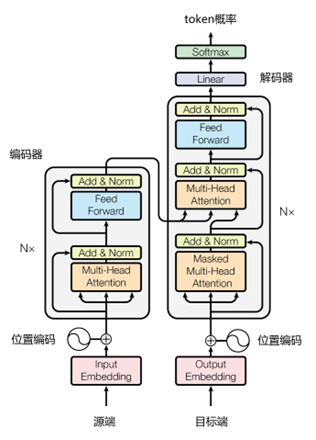
\includegraphics[width=1\textwidth]{figures/Transformer_Structure.png}
	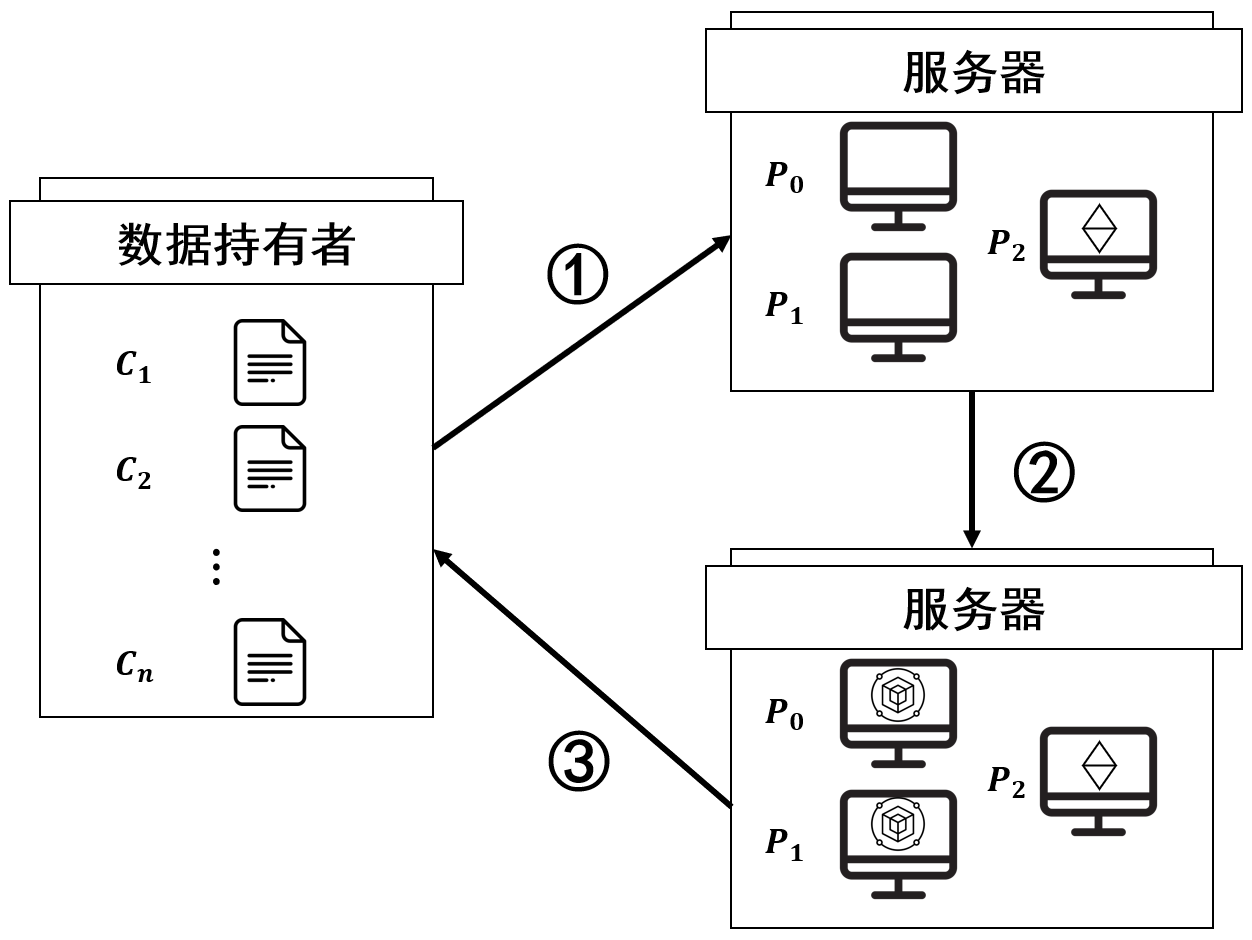
\includegraphics[width=0.75\linewidth]{figures/Chap4_System_Info.png}
	\caption{面向医学文本生成任务训练阶段的系统概述图}
	\label{Chap4_System_Info}
\end{figure}

\subsection{威胁模型与安全假设} \label{chap4ThreatModel}

%本文对该场景下数据持有者的安全假设是其会严格遵循协议提供本地数据并且不会推测其他数据持有者的隐私数据,对计算方的安全假设是其可以任意偏离协议并且会从获取到的数据推断数据持有者的隐私信息以及模型参数,即数据持有者是诚实的,而计算方是恶意的。计算方服务器不仅会根据获取到的信息来推测隐私数据,而且还会任意偏离协议,即在协议执行过程中返回恶意结果。此外,本文假设多个恶意计算方不会共谋。为规范服务器行为,我们引入可信硬件来保障执行过程的完整性。具体来说,本文引入Intel Software Guard Extension(SGX)\cite{SGX_Explained}作为可信硬件。相关研究将SGX视为一个可信第三方,即其机密性与完整性都不被破坏,这样的新人假设过强。由于例如测信道攻击等攻击手段可能会破坏SGX的机密性\cite{SGX_Attack},因此直接将SGX是为一个可信第三方有风险。本协议只关注SGX中Enclave与GPU交互数据时由于访问模式导致的侧信道信息泄露问题,而如缓存冲突攻击、计时攻击和工号分析攻击的其他相关侧信道攻击均不在本方案考虑范围内。本协议对计算方上SGX的信任假设较弱,即其机密性可以被破坏但是会保留其完整性,这是一种对可信硬件常见的安全假设\cite{Cryptflow}。对计算方上GPU的安全假设是其执行内容对服务器可见,但是执行协议不会被破坏。

本文对该场景下数据持有者的安全假设是其会严格遵循协议提供本地数据并且不会推测其他数据持有者的隐私数据,对计算方的安全假设是其可以任意偏离协议并且会从获取到的数据推断数据持有者的隐私信息以及模型参数,即数据持有者是诚实的,而计算方是恶意的。计算方服务器不仅会根据获取到的信息来推测隐私数据,而且还会任意偏离协议,即在协议执行过程中返回恶意结果。此外,本文假设多个恶意计算方不会共谋。为规范服务器行为,本章引入可信硬件来保障执行过程的完整性。具体来说,本文引入Intel SGX\cite{SGX_Explained}作为可信硬件。相关研究将SGX视为一个可信第三方,即其机密性与完整性都不被破坏,这样的信任假设过强。由于测信道攻击等攻击手段可能会破坏SGX的机密性\cite{SGX_Attack},因此直接将SGX是为一个可信第三方有风险。本协议只关注SGX中Enclave与GPU交互数据时由于访问模式导致的侧信道信息泄露问题,而如缓存冲突攻击、计时攻击和工号分析攻击的其他相关侧信道攻击均不在本方案考虑范围内。本协议对计算方上SGX的信任假设较弱,即其机密性可以被破坏但是会保留其完整性,这是一种对可信硬件常见的安全假设\cite{Cryptflow}。对计算方上GPU的安全假设是其执行内容对服务器可见,但是执行协议不会被破坏。


\subsection{设计目标}

对该场景下的安全目标是数据持有者的隐私数据不会被计算方推断出,同时计算方会按照约定的协议严格执行训练过程。


\section{训练协议设计} \label{chap4_train_protocol}

%本节从基于秘密共享的基本的神经网络函数的构建开始,逐渐封装到用于构建大型语言模型模块的实现。
本节从基于秘密共享的基本神经网络函数的构建入手,逐步拓展至用于实现大型语言模型模块的构建和封装。

\subsection{多方安全计算深度学习函数的实现}

%Transformer模型包含线性运算与非线性运算。线性层(Linear Layer)、全连接层(Fully Connected Layer) 、卷积层(Convolutional Layer)本质都是矩阵乘法运算,这是神经网络模型中最经常被用到的运算。模型经常会把这些层通过一些比如ReLU、Sigmoid、Exp等激活函数进行非线性处理。因此,为了构建常见的神经网络模型结构,本文对于这些线性与非线性函数进行了设计。其中,线性运算是矩阵乘法运算。

%本文的非线性运算有ReLU、Softmax与Dropout。其中\cite{SecureNN}\cite{S++}中已经有了ReLU、Tanh、Sigmoid的实现,我们将利用这些函数以及参考\cite{MPC_Fix_Point}中的Trunc、BitDecomp与PreMult函数的实现来构建Exp与Softmax的实现。其中各函数的调用关系如图\ref{Chap4_Func_All}所示,其中标记为红色的是构建模型的主要函数。

Transformer模型包含线性运算与非线性运算。线性层(Linear Layer)、全连接层(Fully Connected Layer) 、卷积层(Convolutional Layer)本质都是矩阵乘法运算,这是神经网络模型中最经常被用到的运算。模型经常会把这些层通过一些比如ReLU、Sigmoid、Exp等激活函数进行非线性处理。因此,为了构建常见的神经网络模型结构,本文对于这些线性与非线性函数进行了设计。其中,线性运算是矩阵乘法运算。

本文的非线性运算有ReLU、Softmax。其中\cite{SecureNN}\cite{S++}中已经有了ReLU、Tanh、Sigmoid的实现,本章将利用这些函数以及参考\cite{MPC_Fix_Point}中的Trunc、BitDecomp与PreMult函数的实现来构建Exp与Softmax的实现。其中各函数的调用关系如图 \ref{Chap4_Func_All} 所示,标记为红色的是构建模型的主要函数。

\begin{figure}[h]
	\centering
	%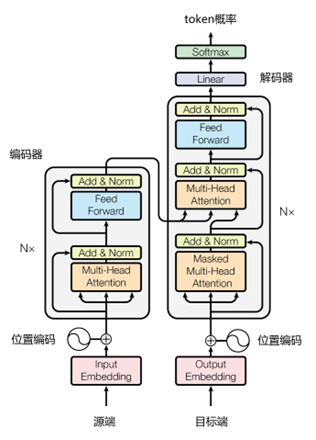
\includegraphics[width=1\textwidth]{figures/Transformer_Structure.png}
	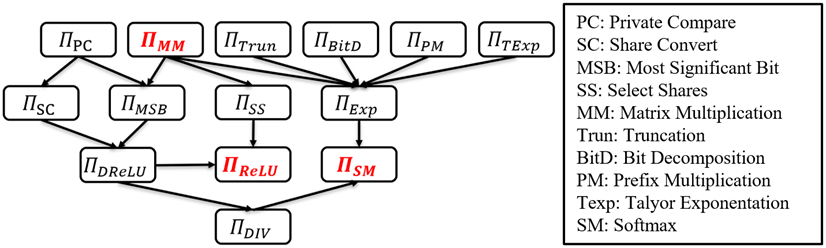
\includegraphics[width=\linewidth]{figures/Chap4_Func_All.png}
	\caption{各函数间的依赖关系}
	\label{Chap4_Func_All}
\end{figure}

算法 \ref{MatMul} 描述了本文的三方矩阵乘法协议($\Pi_{\rm Matmul}(\{P_0, P_1\}, P_2)$),其中参与方$P_0$和$P_1$持有矩阵$X$和$Y$的秘密份额,协议输出$Z=X∙Y$的秘密份额。算法 \ref{Exp} 描述了本文的三方Exp协议($\Pi_{\rm Exp}(\{P_0, P_1\}, P_2)$),其中参与方$P_0$和$P_1$持有矩阵$X$的秘密份额,协议输出$Z=e^X$的秘密份额。有了Exp协议便可以根据其来构建Softmax协议。如算法 \ref{Softmax} 所示,本文的三方Softmax协议($\Pi_{\rm Softmax}(\{P_0, P_1\}, P_2)$)中,参与方$P_0$和$P_1$持有序列 $Z$的秘密份额,协议输出$Z=e^{z_i}/(\sum_{i=1}^k e^{z_i})$的秘密份额。

%\begin{algorithm}[H]
%	%\renewcommand{\thealgocf}{}     %<---细节与重点
%	\SetAlgoLined
%	\SetKwInOut{Input}{输入}
%	\SetKwInOut{Output}{输出}
%	\Input{$P_0$与$P_1$分别持有$(\langle X\rangle_0, \langle Y\rangle_0)$和$(\langle X\rangle_1, \langle Y\rangle_1)$}
%	
%	\Output{对于$i\in \{0, 1\}$, $P_i$获得输出的秘密分片$\langle X \cdot Y\rangle_i$.}
%	
%	$P_0$、$P_1$分别获得从$P_2$产生的$U_0=\langle 0^{m\times n}\rangle_0^L$和$U_1=\langle 0^{m\times n}\rangle_1^L$
%	
%	$P_2$生成随机的矩阵$A\in Z_L^{m\times n}$和$B\in Z_L^{m\times n}$,并计算$C=A\cdot B$。对于$i\in \{0, 1\}$,$P_2$将$A, B, C$分成秘密份额$\langle A\rangle_i^L$, $\langle B\rangle_i^L$, $\langle C\rangle_i^L$,并分发给$P_0$、$P_1$
%	
%	对于$j\in \{0, 1\}$, $P_j$计算$\langle E\rangle_j^L = \langle X\rangle_j^L - \langle A\rangle_j^L$与$\langle F\rangle_j^L = \langle Y\rangle_j^L - \langle B\rangle_j^L$ 
%	
%	$P_0$、$P_1$交换秘密份额来重构$E$与$F$
%	
%	对于$j\in \{0, 1\}$, $P_j$计算$-jE\cdot F + \langle X\rangle_j^L\cdot F + E\cdot \langle Y\rangle_j^L + \langle C\rangle_j^L + U_j$
%	
%	\caption{ $\Pi_{\rm Matmul}(\{P_0, P_1\}, P_2)$ }
%	\label{MatMul}
%\end{algorithm}

\begin{algorithm}[H]
	%\renewcommand{\thealgocf}{} %<---细节与重点
	\SetAlgoLined
	\SetKwInOut{Input}{输入}
	\SetKwInOut{Output}{输出}
	\Input{$P_0$与$P_1$分别持有$(\langle X\rangle_0, \langle Y\rangle_0)$和$(\langle X\rangle_1, \langle Y\rangle_1)$,$X$是$m \times v$的,$Y$是$v \times n$的}
	\Output{对于$i\in \{0, 1\}$, $P_i$获得输出的秘密分片$\langle X \cdot Y\rangle_i$.}
	
	$P_0$、$P_1$分别获得从$P_2$产生的$U_0=\langle 0^{m\times n}\rangle_0^L$和$U_1=\langle 0^{m\times n}\rangle_1^L$
	
	$P_2$生成随机的矩阵$A\in Z_L^{m\times v}$和$B\in Z_L^{v\times n}$,并计算$C=A\cdot B$。对于$i\in \{0, 1\}$,$P_2$将$A, B, C$分成秘密份额$\langle A\rangle_i^L$, $\langle B\rangle_i^L$, $\langle C\rangle_i^L$,并分发给$P_0$、$P_1$
	
	对于$j\in \{0, 1\}$, $P_j$计算$\langle E\rangle_j^L = \langle X\rangle_j^L - \langle A\rangle_j^L$与$\langle F\rangle_j^L = \langle Y\rangle_j^L - \langle B\rangle_j^L$ 
	
	$P_0$、$P_1$交换秘密份额来重构$E$与$F$
	
	对于$j\in \{0, 1\}$, $P_j$计算$-jE\cdot F + \langle X\rangle_j^L\cdot F + E\cdot \langle Y\rangle_j^L + \langle C\rangle_j^L + U_j$
	
	\caption{ $\Pi_{\rm Matmul}(\{P_0, P_1\}, P_2)$ }
	\label{MatMul}
\end{algorithm}

%算法\ref{MatMul}的通信次数计算如下:$P_2$向$P_0$、$P_1$发送三个秘密份额$3$次。$P_0$、$P_1$之间交换秘密份额$2$次。$P_0$、$P_1$分别向$P_2$发送各自的秘密份额$2$次。因此,总共需要 $7$次通信。

%算法\ref{MatMul}的通信复杂度为:$P_2$需要生成两个随机矩阵$A$和$B$,每个矩阵的大小为$m \times v$和$v \times n$,需要$L(mv+vn)$的通信复杂度。$P_2$需要计算矩阵$C=A\cdot B$,需要$L(mnv)$的通信复杂度。$P_0$、$P_1$分别需要计算矩阵$\langle E\rangle_j^L = \langle X\rangle_j^L - \langle A\rangle_j^L$和$\langle F\rangle_j^L = \langle Y\rangle_j^L - \langle B\rangle_j^L$,需要$L(mv)$的通信复杂度。$P_0$、$P_1$需要交换秘密份额以重构矩阵$E$和$F$,需要$L(mv)$的通信复杂度。$P_0$、$P_1$分别需要计算$-jE\cdot F + \langle X\rangle_j^L\cdot F + E\cdot \langle Y\rangle_j^L + \langle C\rangle_j^L + U_j$,需要$L(mn)$的通信复杂度。因此,总通信复杂度为 $O(L(mv+vn+mn))$。

\begin{algorithm}[H]
	%\renewcommand{\thealgocf}{}     %<---细节与重点
	\SetAlgoLined
	\SetKwInOut{Input}{输入}
	\SetKwInOut{Output}{输出}
	\Input{$P_0$与$P_1$分别持有$(\langle x\rangle_0^L)$和$(\langle x\rangle_1^L)$,其中$|x|$ < 1,公开的展开阶数$n$($n \geq 4$)}
	\Output{对于$i\in \{0, 1\}$, $P_i$获得秘密份额$\langle y\rangle_i^L = \langle e^x\rangle_i^L$.}
	
	$P_0$、$P_1$分别获得由$P_2$产生的$u_0=\langle 0\rangle_0^L$和$u_1=\langle 0\rangle_1^L$
	
	$P_0$、$P_1$计算$\langle c\rangle_j^L = j$
	
	$P_0$、$P_1$计算$\langle numerator\rangle_j^L = \langle x\rangle_j^L$并设置$denominator = 1$
	
	$P_0$、$P_1$计算$\langle c\rangle_j^L = \langle c\rangle_j^L + \langle numerator\rangle_j^L$
	
	\For{$i = 2, 3, \cdots, n$}{
		$P_j$的输入为$\langle numerator\rangle_j^L$与$\langle x\rangle_j^L$时,在$P_0$、$P_1$、$P_2$执行$\Pi_{\rm MatMul}(\{P_0, P_1\}, P_2)$后,$P_j$获得$\langle numerator\rangle_j^L = \langle numerator\cdot x\rangle_j^L$
		
		$denominator = denominator\times i$
		
		$P_0$、$P_1$计算$\langle c\rangle_j^L = \langle c\rangle_j^L + \frac{\langle numerator\rangle_j^L}{denominator}$
		
	}
	
	对于$j\in \{0, 1\}$, $P_j$计算$\langle y\rangle_j^L = \langle c\rangle_j^L + u_j$
	\label{TaylorExpansion}
	
	\caption{ $\Pi_{\rm TaylorExpansion}(\{P_0, P_1\}, P_2)$ }
\end{algorithm}

%算法\ref{TaylorExpansion}用于计算$x$的指数$e^x$,其中$|x| < 1$。该算法通过泰勒级数展开来近似$e^x$,并使用$n$阶泰勒级数。这里的$n$是公开的,并且要求$n \geq 4$。通过该算法,参与者$P_0$和$P_1$可以获得$e^x$的秘密份额。该算法利用了$\Pi_{\rm MatMul}({P_0, P_1}, P_2)$协议来实现安全的乘法。在循环中,算法计算泰勒级数的每个项并将其累加到最终结果中。

%为了计算该算法的通信复杂度和通信开销,我们需要关注算法中涉及到的信息交换步骤。我们将重点关注在循环内部执行的$\Pi_{\rm MatMul}({P_0, P_1}, P_2)$协议,因为它是通信成本最高的部分。在$\Pi_{\rm MatMul}({P_0, P_1}, P_2)$协议中,通信复杂度为10次信息传递。由于该协议在循环中执行了$n-1$次(从2到n),因此循环内的总通信复杂度为$10(n-1)$次信息传递。现在,我们来计算通信开销。对于每次$\Pi_{\rm MatMul}({P_0, P_1}, P_2)$调用,通信开销为$10\cdot m \cdot n$。然而,在本算法中,我们只处理单个数值而不是矩阵,因此$m=n=1$。所以,每次$\Pi_{\rm MatMul}({P_0, P_1}, P_2)$调用的通信开销为10。在循环中,$\Pi_{\rm MatMul}({P_0, P_1}, P_2)$被调用了$n-1$次,因此循环内的总通信开销为$10(n-1)$。除了循环内的通信之外,算法还包括在开头和末尾的一些额外通信,但这些通信相对较小,可以忽略。综上所述,$\Pi_{\rm TaylorExpansion}({P_0, P_1}, P_2)$算法的通信复杂度为$10(n-1)$次信息传递,通信开销为$10(n-1)$。这些度量随着泰勒级数展开阶数$n$的增加而线性增加。

\begin{algorithm}[H]
	%\renewcommand{\thealgocf}{}     %<---细节与重点
	\SetAlgoLined
	\SetKwInOut{Input}{输入}
	\SetKwInOut{Output}{输出}
	\Input{$P_0$与$P_1$分别持有$(\langle x\rangle_0^L)$和$(\langle x\rangle_1^L)$}
	
	\Output{对于$i\in \{0, 1\}$, $P_i$获得秘密份额$\langle y\rangle_i^L = \langle e^x\rangle_i^L$.}
	
	$P_0$、$P_1$分别获得由$P_2$产生的$u_0=\langle 0\rangle_0^L$和$u_1=\langle 0\rangle_1^L$
	
	对于$j\in \{0, 1\}$, $P_j$执行$\Pi_{\rm Trunc}(\{P_0, P_1\})$后,获得$\lfloor x \rfloor$的份额$\langle a\rangle_j^L$
	
	对于$j\in \{0, 1\}$, $P_j$通过计算$\langle b\rangle_j^L = \langle x\rangle_j^L - \langle a\rangle_j^L$获得$x$的小数部分$\langle b\rangle_j^L$
	
	对于$j\in \{0, 1\}$, $P_j$执行$\Pi_{\rm BitDecomp}(\{P_0, P_1\})$后,获得$\lfloor x \rfloor$按位展开的秘密份额$(\langle c_0\rangle_j^L, \langle c_1\rangle_j^L, \dots, \langle c_{m-1}\rangle_j^L)$,其中得$\lfloor x \rfloor$是$m$比特数
	
	
	\For{$i = 0, 1, \dots, m-1$}{
		
		对于$j\in \{0, 1\}$, $P_j$计算$\langle v_i\rangle_j^L=e^{2^i}\cdot (\langle c_i\rangle_j^L) + j - (\langle c_i\rangle_j^L)$
		
	}
	
	对于$j\in \{0, 1\}$, $P_j$执行$\Pi_{\rm PreMult}(\{P_0, P_1\})$后,获得$(\langle m\rangle_j^L)$
	
	对于$j\in \{0, 1\}$, $P_j$执行$\Pi_{\rm TaylorExpansion}(\{P_0, P_1\})$后,获得$(\langle n\rangle_j^L)$
	
	对于$j\in \{0, 1\}$, $P_j$的输入为时$(\langle m\rangle_j^L)$与$(\langle n\rangle_j^L)$时,在执行$\Pi_{\rm MatMul}(\{P_0, P_1\}, P_2)$后,$P_j$获得$\langle y\rangle_j^L=\langle m\times n\rangle_j^L$
	
	\caption{ $\Pi_{\rm Exp}(\{P_0, P_1\}, P_2)$ }
	\label{Exp}
\end{algorithm}

算法$\Pi_{\rm Exp}({P_0, P_1}, P_2)$是一个多方安全计算协议,用于计算$x$的指数$e^x$。在该协议中,参与者$P_0$和$P_1$分别持有$x$的秘密份额,并且希望计算$e^x$的秘密份额。此算法利用了算法 \ref{TaylorExpansion} 来近似$e^x$,并利用到前述工作\cite{MPC_Fix_Point}中的子协议,例如$\Pi_{\rm Trunc}({P_0, P_1})$、$\Pi_{\rm BitDecomp}({P_0, P_1})$、$\Pi_{\rm PreMult}({P_0, P_1})$和$\Pi_{\rm TaylorExpansion}({P_0, P_1})$。


\begin{algorithm}[H]
	%\renewcommand{\thealgocf}{}     %<---细节与重点
	\SetAlgoLined
	\SetKwInOut{Input}{输入}
	\SetKwInOut{Output}{输出}
	\Input{$P_0$与$P_1$分别持有$({\langle z_i\rangle_0^L})_{i\in [k]}$和$({\langle z_i\rangle_1^L})_{i\in [k]}$}
	
	\Output{$P_0$,$P_1$分别获得秘密份额$({\langle s_{max}(z_i)\rangle_0^L})_{i\in [k]}$与$({\langle s_{max}(z_i)\rangle_1^L})_{i\in [k]}$,其中$s_{max}(z_i)=\frac{e^{z_i}}{\sum_{i=1}^k e^{z_i}}$.}
	
	$P_0$、$P_1$分别获得由$P_2$产生的$u_0=\langle 0\rangle_0^L$和$u_1=\langle 0\rangle_1^L$
	
	\For{$i = 1, 2, \dots, k$}{
		
		在$P_0$、$P_1$、$P_2$执行$\Pi_{\rm Exp}(\{P_0, P_1\}, P_2)$后,$P_0$,$P_1$分别获得$\langle c_i\rangle_0^L$与$\langle c_i\rangle_1^L$,其中$c_i^L=e^{z_i}$
		
	}
	
	对于$j\in \{0, 1\}$, $P_j$计算$\langle S\rangle_j=\sum_{i=1}^k\langle c_i\rangle_j^L$
	
	\For{$i = 1, 2, \dots, k$}{
		
		在$P_0$、$P_1$、$P_2$执行$\Pi_{\rm Division}(\{P_0, P_1\}, P_2)$后,$P_0$,$P_1$分别获得$\langle \frac{c_i}{S}\rangle_0^L$与$\langle \frac{c_i}{S}\rangle_1^L$
		
		对于$j\in \{0, 1\}$, $P_j$计算$({\langle s_{max}(z_i)\rangle_1^L})_{i\in [k]} + u_j$
	}
	
	\caption{ $\Pi_{\rm Softmax}(\{P_0, P_1\}, P_2)$ }
	\label{Softmax}
\end{algorithm}

在算法 \ref{Softmax} 中,$P_0$和$P_1$分别持有$k$个数值的秘密份额,其主要目标是计算Softmax函数,即对每个$i$,算法得到$s_{max}(z_i) = \frac{e^{z_i}}{\sum_{i=1}^k e^{z_i}}$的秘密份额。首先,$P_0$和$P_1$分别获得由$P_2$产生的零值份额$u_0=\langle 0\rangle_0^L$和$u_1=\langle 0\rangle_1^L$。对于每个$i$,使用$\Pi_{\rm Exp}({P_0, P_1}, P_2)$算法计算指数值$e^{z_i}$的秘密份额$\langle c_i\rangle_0^L$和$\langle c_i\rangle_1^L$。接着,$P_0$和$P_1$计算总和$S$的秘密份额$\langle S\rangle_j=\sum_{i=1}^k\langle c_i\rangle_j^L$。再对于每个$i$,通过$\Pi_{\rm Division}({P_0, P_1}, P_2)$算法计算$\frac{c_i}{S}$的秘密份额$\langle \frac{c_i}{S}\rangle_0^L$和$\langle \frac{c_i}{S}\rangle_1^L$。最后,$P_0$和$P_1$将结果加上零值份额$u_j$以获得$s_{max}(z_i)$的秘密份额。

%通信复杂度和通信开销分析:$\Pi_{\rm Exp}({P_0, P_1}, P_2)$算法需要进行$k$次调用。假设每次调用的通信复杂度为$O(E)$,那么总通信复杂度为$O(kE)$。$\Pi_{\rm Division}({P_0, P_1}, P_2)$算法也需要进行$k$次调用。假设每次调用的通信复杂度为$O(D)$,那么总通信复杂度为$O(kD)$。其他操作,如加法和求和,的通信复杂度较低,可以认为是$O(k)$。综上,整个算法的通信复杂度为$O(kE + kD + k) = O(k(E + D + 1))$。由于$E$和$D$通常较大,通信开销主要取决于这两个基本操作的次数$k$。如果$k$很大,通信开销可能会相应增加。但是,在许多应用场景中,$k$通常是一个较小的值,因此整个算法的通信开销在许多应用场景中仍然是可接受的。

\subsection{语言模型模块的构建} \label{trans_block}

在第 \ref{chap4_train_protocol} 节中,本章介绍了神经网络基本函数的设计。接下来,本节将介绍如何构建语言模型 Transformer 编码器中的各个模块。具体而言,我们将从线性层 Linear、注意力层 Attention 和前馈网络 FFN 这三个模块的构建进行介绍。

\begin{algorithm}[H]
	%\renewcommand{\thealgocf}{}     %<---细节与重点
	\SetAlgoLined
	\SetKwInOut{Input}{输入}
	\SetKwInOut{Output}{输出}
	\Input{$P_0$与$P_1$分别持有$(\langle X\rangle_0, \langle W\rangle_0, \langle b\rangle_0)$和$(\langle X\rangle_1, \langle W\rangle_1, \langle b\rangle_1)$}
	
	\Output{对于$i\in \{0, 1\}$, $P_i$获得输出的秘密分片$\langle W\cdot X + b\rangle_i$.}
	
	$P_0$、$P_1$分别获得从$P_2$产生的$U_0=\langle 0^{m\times n}\rangle_0^L$和$U_1=\langle 0^{m\times n}\rangle_1^L$
	
	在$P_0$、$P_1$、$P_2$执行$\Pi_{\rm Matmul}(\{P_0, P_1\}, P_2)$后,$P_0$,$P_1$分别获得$\langle W\cdot X\rangle_0^L$与$\langle W\cdot X\rangle_1^L$
	
	对于$j\in \{0, 1\}$, $P_j$计算$\langle y\rangle_i^L = \langle W\cdot X\rangle_i^L + \langle b\rangle_i^L$
	
	\caption{ $\Pi_{\rm Linear}(\{P_0, P_1\}, P_2)$ }
	\label{Linear}
\end{algorithm}

算法 \ref{Linear} 在 $\Pi_{\rm Matmul}({P_0, P_1}, P_2)$ 协议的基础上引入了偏置项(Bias),从而将 $\langle W\cdot X\rangle_i$ 扩展到了 $\langle W\cdot X + b\rangle_i$,以实现Linear模块。Linear模块作为整个模型中最基础的模块之一,其设计和实现将在后续的模块设计中被频繁调用。

\begin{algorithm}[H]
	%\renewcommand{\thealgocf}{}     %<---细节与重点
	\SetAlgoLined
	\SetKwInOut{Input}{输入}
	\SetKwInOut{Output}{输出}
	\Input{$P_0$与$P_1$分别持有$(\langle X\rangle_0, \langle W_Q\rangle_0, \langle b_Q\rangle_0, \langle W_K\rangle_0, \langle b_K\rangle_0, \langle W_V\rangle_0, \langle b_V\rangle_0, \langle W_P\rangle_0, \langle b_P\rangle_0)$和$(\langle X\rangle_1, \langle W_Q\rangle_1, \langle b_Q\rangle_1, \langle W_K\rangle_1, \langle b_K\rangle_1, \langle W_V\rangle_1, \langle b_V\rangle_1, \langle W_P\rangle_1, \langle b_P\rangle_1)$}
	
	\Output{对于$i\in \{0, 1\}$, $P_i$获得输出的秘密分片$\langle W_P\cdot Softmax(\frac{ (W_Q\cdot X + b_Q)(W_K\cdot X + b_K)^T }{\sqrt[]{d_k}})(W_V\cdot X + b_V) + b_P\rangle_i$.}
	
	$P_0$、$P_1$、$P_2$执行$\Pi_{\rm Linear}(\{P_0, P_1\}, P_2)$,$P_0$、$P_1$分别获得$Q=W_Q\cdot X + b_Q$, $K=W_K\cdot X + b_K$, $V=W_V\cdot X + b_V$的秘密份额($\langle Q\rangle_0$, $\langle K\rangle_0$, $\langle V\rangle_0$)与($\langle Q\rangle_1$, $\langle K\rangle_1$, $\langle V\rangle_1$)
	
	$P_0$、$P_1$分别将$\langle K\rangle_0$与$\langle K\rangle_1$转置得到$\langle K^T\rangle_0$与$\langle K^T\rangle_1$
	
	$P_0$、$P_1$、$P_2$执行$\Pi_{\rm MatMul}(\{P_0, P_1\}, P_2)$,$P_0$、$P_1$分别获得$QK^T$的秘密份额$\langle QK^T\rangle_0$与$\langle QK^T\rangle_1$
	
	$P_0$、$P_1$分别将$\langle QK^T\rangle_0$与$\langle QK^T\rangle_1$按元素除$W_K$的维度$\sqrt[]{d_k}$得到$\langle\frac{ QK^T }{\sqrt[]{d_k}}\rangle_0$与$\langle\frac{ QK^T }{\sqrt[]{d_k}}\rangle_1$
	
	$P_0$、$P_1$、$P_2$执行$\Pi_{\rm Softmax}(\{P_0, P_1\}, P_2)$,$P_0$、$P_1$分别获得$A=\text{Softmax}(\frac{ QK^T }{\sqrt[]{d_k}})$的秘密份额$\langle A\rangle_0$与$\langle A\rangle_1$
	
	$P_0$、$P_1$、$P_2$执行$\Pi_{\rm Linear}(\{P_0, P_1\}, P_2)$,$P_0$、$P_1$分别获得$\langle A\cdot V + b_V\rangle_0$与$\langle A\cdot V + b_V\rangle_1$
	
	$P_0$、$P_1$、$P_2$执行$\Pi_{\rm Linear}(\{P_0, P_1\}, P_2)$,$P_0$、$P_1$分别获得$\langle y\rangle_0 = \langle W_P(A\cdot V + b_V) + b_P\rangle_0$与$\langle y\rangle_1 = \langle W_P(A\cdot V + b_V) + b_P\rangle_1$
	
	\caption{ $\Pi_{\rm Attention}(\{P_0, P_1\}, P_2)$ }
	\label{Attention}
\end{algorithm}

算法 \ref{Attention} 展示了在 $\Pi_{\rm Linear}({P_0, P_1}, P_2)$ 和 $\Pi_{\rm MatMul}({P_0, P_1}, P_2)$ 协议的基础上如何构建注意力机制(Attention)。该算法提供了对输入 $\langle X\rangle_i$ 进行注意力变换后的秘密共享结果,其输出为 $\langle W_P\cdot \text{Softmax}(\frac{ (W_Q\cdot X + b_Q)(W_K\cdot X + b_K)^T }{\sqrt[]{d_k}})(W_V\cdot X + b_V) + b_P\rangle_i$。

该算法中,注意力变换首先对输入 $\langle X\rangle_i$ 分别进行三次线性变换,得到 $Q=W_Q\cdot X + b_Q$,$K=W_K\cdot X + b_K$ 和 $V=W_V\cdot X + b_V$。然后,算法利用了线性模块进行计算,得到 $QK^T$,并将其除以 $\sqrt[]{d_k}$ 进行缩放。这个缩放过程使得模型在进行自注意力计算时能更好地保持稳定性。接下来,算法对缩放后的结果进行 Softmax 变换,得到注意力分布 $A=\text{Softmax}(\frac{ QK^T }{\sqrt[]{d_k}})$。然后,将注意力分布与 $V$ 进行乘积运算,并加上偏置项 $b_V$。最后,算法对上一步得到的结果再进行一次线性变换,得到最终的输出 $\langle y\rangle_i = \langle W_P(A\cdot V + b_V) + b_P\rangle_i$。

注意力机制是 Transformer 中的核心组成部分,它允许模型在处理序列数据时,对输入数据中的不同部分分配不同的注意力权重。通过这种方式,模型可以更好地理解和表示序列中的依赖关系。这个 $\Pi_{\rm Attention}({P_0, P_1}, P_2)$ 算法正是基于这种思想,将注意力机制融入到大型语言模型的构建过程中,从而提升模型的表达能力。

\begin{algorithm}[H]
	%\renewcommand{\thealgocf}{}     %<---细节与重点
	\SetAlgoLined
	\SetKwInOut{Input}{输入}
	\SetKwInOut{Output}{输出}
	\Input{$P_0$与$P_1$分别持有$(\langle X\rangle_0, \langle W_1\rangle_0, \langle W_2\rangle_0, \langle b_1\rangle_0, \langle b_2\rangle_0)$和$(\langle X\rangle_1, \langle W_1\rangle_1, \langle W_2\rangle_1, \langle b_1\rangle_1, \langle b_2\rangle_1)$}
	
	\Output{对于$i\in \{0, 1\}$, $P_i$获得输出的秘密分片$\langle W_2\cdot \text{ReLU}(W_1\cdot X + b_1) + b_2\rangle_i$.}
	
	$P_0$、$P_1$分别获得从$P_2$产生的$U_0=\langle 0^{m\times n}\rangle_0^L$和$U_1=\langle 0^{m\times n}\rangle_1^L$
	
	
	
	$P_j$的输入为$\langle X\rangle_j^L$与$\langle W_1\rangle_j^L$时,在$P_0$、$P_1$、$P_2$执行$\Pi_{\rm Linear}(\{P_0, P_1\}, P_2)$后,$P_j$获得$\langle H\rangle_j^L = \langle W_1\cdot X + b_1\rangle_j^L$ 
	
	在$P_0$、$P_1$、$P_2$执行$\Pi_{\rm ReLU}(\{P_0, P_1\}, P_2)$后,$P_j$获得$\langle \text{ReLU}(H)\rangle_j^L$ 
	
	$P_j$的输入为$\langle \text{ReLU}(H)\rangle_j^L$与$\langle W_2\rangle_j^L$时,在$P_0$、$P_1$、$P_2$执行$\Pi_{\rm Linear}(\{P_0, P_1\}, P_2)$后,$P_j$获得$\langle O\rangle_j^L = \langle W_2\cdot \text{ReLU}(H) + b_2 \rangle_j^L$ 
	
	对于$j\in \{0, 1\}$, $P_j$计算$\langle O\rangle_j^L + U_j$
	
	\caption{ $\Pi_{\rm FFN}(\{P_0, P_1\}, P_2)$ }
	\label{FFN}
\end{algorithm}

算法 \ref{FFN} 表示的是一个前馈神经网络的计算过程,其中包含了两个线性(Linear)变换和一个ReLU激活函数。在算法执行过程中,首先在 $\Pi_{\rm Linear}({P_0, P_1}, P_2)$ 协议的基础上对输入 $X$ 进行第一次线性变换,即乘以权重 $W_1$ 并加上偏置 $b_1$,获得 $H$,然后将 $H$ 通过ReLU激活函数进行非线性变换。ReLU函数的作用是将所有负数变为0,对所有正数保持不变,其计算公式为:$\text{ReLU}(x) = \max(0, x)$。这个操作是在 $\Pi_{\rm ReLU}({P_0, P_1}, P_2)$ 协议中进行的。接着,对ReLU激活后的结果进行第二次线性变换,即乘以权重 $W_2$ 并加上偏置 $b_2$,得到 $O$。最后,$P_0$ 和 $P_1$ 对各自得到的结果进行一次局部计算,即与零矩阵的份额 $U_j$ 相加,得到最终的结果 $\langle O\rangle_j^L$。

FFN模块是神经网络中的一个基本模块,其功能是在保持输入和输出的维度不变的同时,对输入进行复杂的非线性变换,从而增加模型的表达能力。在多层神经网络中,通常会使用多个此类模块进行堆叠,以构建更深的网络结构。

\subsection{可验证外包计算的设计}

本节介绍了一个可验证外包计算的设计,与前一部分不同的是,此设计需要每个服务器都拥有高性能的GPU计算资源。回顾 \ref{chap4ThreatModel} 节中的安全假设,本章假设计算方是恶意的,可以任意偏离协议并推断数据持有者的隐私信息和模型参数。对于计算方上的SGX,本章假设其机密性可能被破坏但会保留其完整性;对于计算方上的GPU,本章假设其执行内容对服务器可见,但执行协议不会被破坏。这是一种对可信硬件常见的安全假设\cite{Cryptflow}。

如图 \ref{Chap4_With_GPU} 所示,首先,数据持有者使用秘密共享方法将数据拆分成两个秘密份额,并在与两个服务器的可信硬件进行远程认证后,将数据分发至服务器。然后,在与第三个持有可信硬件的服务器认证后,服务器之间根据算法的具体实现方式进行交互。两个获得秘密份额的服务器在第三个服务器提供的随机数的帮助下,完成相应的算法计算。最终,两个服务器分别得到的预测结果的秘密份额,在交互重构后得到最终的预测结果,并通过真值计算损失函数来更新存储在两个服务器上的权重。


\begin{figure}[h]
	\centering
	%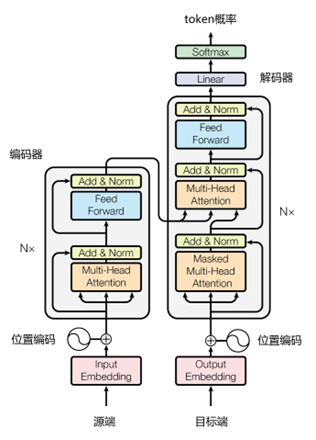
\includegraphics[width=1\textwidth]{figures/Transformer_Structure.png}
	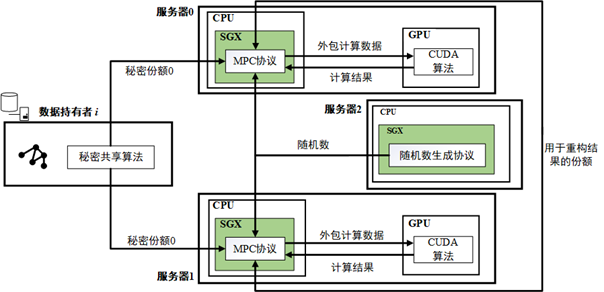
\includegraphics[width=\linewidth]{figures/Chap4_With_GPU.png}
	\caption{外包计算的协议流程}
	\label{Chap4_With_GPU}
\end{figure}


\begin{algorithm}[H]
	%\renewcommand{\thealgocf}{}     %<---细节与重点
	\SetAlgoLined
	\SetKwInOut{Input}{输入}
	\SetKwInOut{Output}{输出}
	\Input{SGX持有模型矩阵参数$M$的秘密份额$\langle M\rangle_j^L \in Z_L^{m\times d}$与输入$x$的秘密份额$\langle x\rangle_j^L \in Z_L^{d\times n}$}
	
	\Output{SGX获得计算结果$\langle M\rangle_j^L\cdot \langle x\rangle_j^L$}
	
	SGX将$\langle M\rangle_j^L$与$\langle x\rangle_j^L$分发给GPU
	
	GPU计算$y = \langle M\rangle_j^L\cdot \langle x\rangle_j^L$
	
	\For{$i = 1, 2, \dots, n$}{
		
		SGX生成随机向量$\alpha \in Z_L^{n\times 1}$
		
		SGX验证$y\cdot \alpha$与$\langle M\rangle_j^L \cdot (\langle x\rangle_j^L \cdot \alpha)$是否相等
		
	}
	
	\caption{外包计算并验证正确性}
	\label{outalg}
\end{algorithm}

%算法\ref{OutsourceGPU}描述了本文的外包计算协议。SGX先将需要计算的秘密份额分发给本地的GPU,在GPU计算完结果返回给SGX后,SGX执行Freivalds' 验证\cite{Random_Algorithm}算法来校验计算结果的正确性。其中,Freivalds' 验证算法是一种概率算法,为了验证矩阵运算$A∙B=C$的正确性。其通过引入一个列向量$x$,分别计算$A∙(B∙x)$与$C∙x$的结果是否相等来验证正确性。由于矩阵与列向量的运算时间短,从而将验证的时间由$O(n^3)$降至$O(kn^2)$,其中$k$为验证次数。

算法 \ref{outalg} 描述了本文的外包计算协议。为了加速计算,本文引入了GPU并进行了外包计算。具体来说,SGX将需要计算的秘密份额分发给本地的GPU,GPU计算完结果后返回给SGX。然后,SGX使用Freivalds'验证算法\cite{Random_Algorithm}来校验计算结果的正确性。该算法通过引入一个列向量$x$,计算$A∙(B∙x)$与$C∙x$的结果,来验证矩阵运算$A∙B=C$的正确性。由于矩阵与列向量的运算时间短,该验证算法能将验证时间由$O(n^3)$降至$O(kn^2)$,其中$k$为验证次数。因此,Freivalds' 验证算法确保了外包计算的正确性,而秘密共享技术则保护了数据的隐私,整体实现了计算过程的隐私保护和计算正确性验证。

\section{安全性分析}


\subsection{训练安全}

基于通用可组合模型\cite{Universally_Compsable, Simple_UC}(Universally Compsable,UC),本部分给出 \ref{chap4_train_protocol} 中各算法的系统安全性的理论证明。根据 \ref{chap2_system_model} 的定义,本部分证明本章的系统在恶意攻击者存在的情况下能够保证安全性。在 \ref{chap2_system_model} 的安全假设中,假设存在一个敌手A,它能够控制其中一个参与方。令$I\subset N$表示被控制方的集合,$|I|=1$。设$J = N / I$是诚实的参与者的集合。在整个证明过程中,$P_i  (i∈I)$表示被攻击者操作一方,而$P_j  (j∈J)$表示诚实方。安全性定义遵循相关工作中的方法。与研究工作\cite{SecureNLP, Sim_Proof, Sharemind}相同,在本章条件下有如下引理成立:

\begin{definition}{}
	对于任何多项式时间的攻击者A,如果存在一个模拟器S能够构建一个模拟世界,在这个模拟世界中A的视图与真实世界中A的视图在计算上不可区分,那么该协议是可证明安全的。
\end{definition}


\begin{lemma}
	如果一个协议的所有子协议都是完全可模拟的,那么该协议本身也是完全可模拟的。
\end{lemma}


在UC框架中,一个协议通常由多个子协议组成,每个子协议都有自己的安全性质。如果每个子协议都是可模拟的,也就是说,每个子协议都可以在模拟环境中与理想功能模型等效地运行,那么整个协议也可以在模拟环境中与理想功能模型等效地运行。

这是因为在UC框架中,可以使用虚拟攻击者来证明协议的安全性,虚拟攻击者在真实环境和模拟环境下执行相同的攻击,然后证明模拟环境中的协议能够抵御虚拟攻击者的攻击。如果每个子协议都是可模拟的,那么整个协议也可以在模拟环境中与理想功能模型等效地运行,因此整个协议也可以被证明是安全的。%因此,如果一个协议的所有子协议都是可模拟的,那么该协议本身也可以被证明是可模拟的。

\begin{lemma}
	如果$r$是攻击者未知的且服从均匀分布的一个随机数,那么$x\cdot r$对攻击者也是未知的,并且与$x$独立。
\end{lemma}

\begin{lemma} \label{ss_pm}
	如果$r$是攻击者未知的且服从均匀分布的一个随机数,那么$x\pm r$对攻击者也是未知的,并且与$x$独立。
\end{lemma}

\begin{lemma} \label{ss_matmul}
	$\Pi_{\rm Matmul}(\{P_0, P_1\}, P_2)$以及其线性组合是安全的\cite{Threshold_ECDSA, beaver_efficient}。
\end{lemma}

\begin{lemma} \label{ss_trunc_Bit_premult}
	$\Pi_{\rm Trunc}(\{P_0, P_1\})$、$\Pi_{\rm BitDecomp}(\{P_0, P_1\})$、$\Pi_{\rm PreMult}(\{P_0, P_1\})$是可模拟的\cite{fix_point_mpc}
\end{lemma}

基于上述的引理,下面本节提供 \ref{chap4_train_protocol} 中各算法的系统安全性的理论证明,即存在模拟器S使得攻击者A在现实世界与理想世界中的视图在计算上是不可区分的。

\begin{theorem}
	\label{TayRxp_theorem}
	在 \ref{chap2_system_model} 中的安全假设下,$\Pi_{\rm TaylorExpansion}(\{P_0, P_1\}, P_2)$可以保证面对恶意攻击者攻击的安全性。
\end{theorem}

%\renewcommand{\qedsymbol}{}
\begin{proof}
	\begin{itemize}
		\item [1)$a$]
		%\item [$a$]
		若$P_i=P_0$或$P_i=P_1$,其持有数据的视图如下:
		$$view_i^{\text{TaylorExpansion}}=\{u_i, \langle x\rangle_i,\langle numerator\rangle_i, denominator, \langle c\rangle_i\}\text{,}$$
		$$output_i^{\text{TaylorExpansion}}=\{y_i\}\text{,}$$
		%\hspace{2em}
		其中秘密份额$\langle x\rangle_i$的安全性由引理 \ref{ss_pm} 保障。根据引理 \ref{ss_matmul},现有工作已证明$\Pi_{\rm Matmul}(\{P_0, P_1\}, P_2)$在半诚实攻击者存在情况下的安全性,因此在以$\langle x\rangle_i$作为输入的情况下,$\langle numerator\rangle_i$的值满足均匀随机性。此外,由于$denominator$是每一阶Talor Expansion的常系数,与$x$无关。在以$\langle numerator\rangle_i$与$denominator$作为输入的$\langle c\rangle_i$同样满足均匀随机性。至此,模拟器可以使用均匀分布的随机数来模拟$view_i^{\text{TaylorExpansion}}$,即攻击者的模拟视图与现实视图的概率分布不可区分。对于计算结果$output_i^{\text{TaylorExpansion}}=\{y_i\}$,$x$为加法秘密共享$\langle x\rangle_i$的重构值,由计算过程$c$为计算$x$的$n$阶Taylor展开值的加法秘密共享$\langle c\rangle_i$的秘密份额,因此输出$\langle y\rangle_j^L = \langle c\rangle_j^L + u_j$满足均匀随机性,并且重构结果等于正确的计算结果,故模拟器可以通过满足均匀分布的随机数与理想功能的输出对$output_i^{\text{TaylorExpansion}}=\{y_i\}$进行有效模拟,即其输出的概率分布与真实世界的输出满足不可区分性。至此,证明了$\Pi_{\rm TaylorExpansion}(\{P_0, P_1\}, P_2)$可抵抗半诚实攻击者。
		
		\item [$b$]
		若$P_i=P_2$,其持有数据的视图为:
		$$view_i^{\text{TaylorExpansion}}=\{u_0^s, u_1^s, \langle A\rangle_i^s,\langle B\rangle_i^s,\langle C\rangle_i^s, A^s, B^s, C^s\}\text{,}$$
		$$output_i^{\text{TaylorExpansion}}=\{u_0^s, u_1^s\, \langle A\rangle_i^s,\langle B\rangle_i^s,\langle C\rangle_i^s\}\text{,}$$
	
		其中$s$为$\Pi_{\rm TaylorExpansion}(\{P_0, P_1\}, P_2)$中调用$\Pi_{\rm Matmul}(\{P_0, P_1\}, P_2)$的场景。$P_2$在整个过程中只对$P_0, P_1$单向提供$\Pi_{\rm Matmul}(\{P_0, P_1\}, P_2)$计算所需随机数,故不会获取任何有关$x$的任何信息。由于$u_0^s, A^s, B^s, \langle A\rangle_0^s,\langle B\rangle_0^s,\langle C\rangle_0^s$为$P_2$独立生成的随机数,在半诚实的场景下,其计算的$u_1^s, C^s, \langle A\rangle_1^s,\langle B\rangle_1^s,\langle C\rangle_1^s$均满足均匀随机性,并且$\{(u_0^s, u_1^s), (\langle A\rangle_0^s, \langle A\rangle_1^s), (\langle B\rangle_0^s, \langle B\rangle_1^s), (\langle C\rangle_0^s, \langle C\rangle_1^s)\}$可分别重构为$\{0, A, B, C\}$,故模拟器可以通过满足均匀分布的随机数与理想功能的输出对$output_i^{\text{TaylorExpansion}}$进行有效模拟,其输出的概率分布与真实世界的输出满足不可区分性。
		
		\item [2)]
		
		同时,在 \ref{chap2_system_model} 中的安全假设下,由于SGX的完整性保障\cite{SGX_Explained},$P_i$无法对SGX飞地内的数据进行篡改,即将上述半诚实攻击者升级为恶意攻击者时,协议仍可以保障攻击者严格遵守协议。因此,恶意攻击者不仅推断不出隐私数据,而且不能偏离协议执行其他操作,即本协议可以抵御恶意攻击者的攻击。
		
		因此,$view_i^{\text{TaylorExpansion}}$是可模拟的,无法找到一个概率多项式时间算法来区分$view_i$和$P_i$的模拟视图。因此,$\Pi_{\rm TaylorExpansion}(\{P_0, P_1\}, P_2)$在 \ref{chap2_system_model} 中的安全假设下是安全的。
		
	\end{itemize}

%	若$P_i=P_0$或$P_i=P_1$,其持有数据的视图为:
%	
%	$$view_i^{TaylorExpansion}=\{u_i, \langle x\rangle_i,\langle numerator\rangle_i, denominator, \langle c\rangle_i\}$$
%	
%	$$output_i^{TaylorExpansion}=\{y_i\}$$
%	
%	其中秘密份额$\langle x\rangle_i$的安全性由\ref{ss_pm}保障。根据引理\ref{ss_matmul},现有工作已证明$\Pi_{\rm Matmul}(\{P_0, P_1\}, P_2)$在半诚实攻击者存在情况下的安全性,因此在以$\langle x\rangle_i$作为输入的情况下,$\langle numerator\rangle_i$的值满足均匀随机性。此外,由于$denominator$是每一阶Talor Expansion的常系数,与$x$无关。在以$\langle numerator\rangle_i$与$denominator$作为输入的$\langle c\rangle_i\}$同样满足均匀随机性。至此,模拟器可以使用均匀分布的随机数来模拟$view_i^{TaylorExpansion}$,即攻击者的模拟视图与现实视图的概率分布不可区分。对于计算结果$output_i^{TaylorExpansion}=\{y_i\}$,$x$为加法秘密共享$\langle x\rangle_i\}$的重构值,由计算过程$c$为计算$x$的$n$阶Taylor展开值的加法秘密共享$\langle c\rangle_i\}$的秘密份额,因此输出$\langle y\rangle_j^L = \langle c\rangle_j^L + u_j$满足均匀随机性,并且重构结果满足等于正确计算结果,故$output_i^{TaylorExpansion}=\{y_i\}$可以通过满足均匀分布的随机数与理想功能的输出对计算结果进行有效模拟,其输出的概率分布与真实世界的输出满足不可区分性。至此,$\Pi_{\rm TaylorExpansion}(\{P_0, P_1\}, P_2)$可抵抗半诚实攻击者。
%	
%	若$P_i=P_2$,其持有数据的视图为:
%	
%	$$view_i^{TaylorExpansion}=\{u_0^s, u_1^s, \langle A\rangle_i^s,\langle B\rangle_i^s,\langle C\rangle_i^s, A^s, B^s, C^s\}$$
%	
%	$$output_i^{TaylorExpansion}=\{u_0^s, u_1^s\, \langle A\rangle_i^s,\langle B\rangle_i^s,\langle C\rangle_i^s\}$$
%
%	其中$s$为$\Pi_{\rm TaylorExpansion}(\{P_0, P_1\}, P_2)$中调用$\Pi_{\rm Matmul}(\{P_0, P_1\}, P_2)$的场景。$P_2$在整个过程中只对$P_0, P_1$单向提供$\Pi_{\rm Matmul}(\{P_0, P_1\}, P_2)$计算所需随机数,故不会获取任何有关$x$的任何信息。由于$u_0^s, A^s, B^s, \langle A\rangle_0^s,\langle B\rangle_0^s,\langle C\rangle_0^s$为$P_2$独立生成的随机数,在半诚实的场景下,其计算的$u_1^s, C^s, \langle A\rangle_1^s,\langle B\rangle_1^s,\langle C\rangle_1^s$均满足均匀随机性,并且$\{(u_0^s, u_1^s), (\langle A\rangle_0^s, \langle A\rangle_1^s), (\langle B\rangle_0^s, \langle B\rangle_1^s), (\langle C\rangle_0^s, \langle C\rangle_1^s)\}$可分别重构为$\{0, A, B, C\}$,故$output_i^{TaylorExpansion}$可以通过满足均匀分布的随机数与理想功能的输出对计算结果进行有效模拟,其输出的概率分布与真实世界的输出满足不可区分性。
%	
%	同时,由于SGX的完整性保障,$P_i$无法对SGX飞地内的数据进行篡改。因此,$view_i$是可模拟的,无法找到一个概率多项式时间算法来区分$view_i$和$P_i$的模拟视图。因此,$\Pi_{\rm Exp}(\{P_0, P_1\}, P_2)$在2.1中的安全假设下是安全的。
%	
%	与定理2.1类似,我们可以证明$\Pi_{\rm Softmax}(\{P_0, P_1\}, P_2)$在2.1中的安全假设下是安全的。%因此,由引理2.1可知,模块Π_Attention与Π_FFN在2.1的威胁模型下是安全的。
%	
\end{proof}

\begin{theorem}
	\label{Exp_theorem}
	在 \ref{chap2_system_model} 中的安全假设下,$\Pi_{\rm Exp}(\{P_0, P_1\}, P_2)$可以保证面对恶意攻击者攻击的安全性。
\end{theorem}

%\renewcommand{\qedsymbol}{}
\begin{proof}
	若$P_i=P_0$或$P_i=P_1$,其持有数据的视图如下:
	$$view_i^{\text{Exp}}=\{u_i, \langle x\rangle_i,\langle a\rangle_i, \langle b\rangle_i, \langle c[0],\cdots, c[m-1]\rangle_i,\langle m\rangle_i,\langle n\rangle_i\}\text{,}$$
	$$output_i^{\text{Exp}}=\{y_i\}\text{,}$$
	
	其中秘密份额$\langle x\rangle_i$的安全性由引理 \ref{ss_pm} 保障。引理 \ref{ss_trunc_Bit_premult} 保障了$\langle a\rangle_i=\langle \lfloor x \rfloor \rangle$的安全性,进而获得$x$的小数部分$\langle b\rangle_j^L = \langle x\rangle_j^L - \langle a\rangle_j^L$满足均匀随机性。同样的,在执行$\Pi_{\rm BitDecomp}(\{P_0, P_1\})$获得的$\langle c[0],\cdots, c[m-1]\rangle_i$以及执行$\Pi_{\rm PreMult}(\{P_0, P_1\})$获得的$\langle m\rangle_i$也满足均匀随机性。根据定理 \ref{TayRxp_theorem},TaylorExpansion的计算结果$\langle n\rangle_i$满足均匀随机性。根据引理 \ref{ss_matmul},现有工作已证明$\Pi_{\rm Matmul}(\{P_0, P_1\}, P_2)$在半诚实攻击者存在情况下的安全性,因此在以$\langle m\rangle_i$与$\langle n\rangle_i$作为输入的情况下,$\langle y\rangle_i$的值满足均匀随机性,并且重构结果等于正确的计算结果,故模拟器可以通过满足均匀分布的随机数与理想功能的输出对$output_i^{\text{Exp}}=\{y_i\}$进行有效模拟,其输出的概率分布与真实世界的输出满足不可区分性。至此,证明了$\Pi_{\rm Exp}(\{P_0, P_1\}, P_2)$可抵抗半诚实攻击者。
	
	与定理 \ref{TayRxp_theorem} 的证明相同,同理可证在$P_i=P_2$时,模拟器可以通过满足均匀分布的随机数与理想功能的输出对$view_i^{\text{Exp}}$与$output_i^{\text{Exp}}$进行有效模拟,其输出的概率分布与真实世界的输出满足不可区分性。
	
	同样的,在 \ref{chap2_system_model} 中的安全假设下,由于SGX的完整性保障\cite{SGX_Explained},$P_i$无法对SGX飞地内的数据进行篡改,即将上述半诚实攻击者升级为恶意攻击者时,协议仍可以保障攻击者严格遵守协议。因此,恶意攻击者不仅推断不出隐私数据,而且不能偏离协议执行其他操作,即本协议可以抵御恶意攻击者的攻击。
	
	因此,$view_i^{\text{Exp}}$是可模拟的,无法找到一个概率多项式时间算法来区分$view_i$和$P_i$的模拟视图。因此,$\Pi_{\rm Exp}(\{P_0, P_1\}, P_2)$在 \ref{chap2_system_model} 中的安全假设下是安全的。
	
\end{proof}



\begin{theorem}
	\label{Linear_theorem}
	在 \ref{chap2_system_model} 中的安全假设下,$\Pi_{\rm Linear}(\{P_0, P_1\}, P_2)$可以保证面对恶意攻击者攻击的安全性。
\end{theorem}

\begin{proof}
	若$P_i=P_0$或$P_i=P_1$,其持有数据的视图如下:
	
	$$view_i^{\text{Linear}}=\{u_i, \langle X\rangle_i,\langle W\rangle_i, \langle b\rangle_i\}\text{,}$$
	$$output_i^{\text{Linear}}=\{y_i\}\text{,}$$
	其中秘密份额$\langle X\rangle_i$与权重矩阵$\langle W\rangle_i$的安全性由 \ref{ss_pm} 保障。根据引理 \ref{ss_matmul},现有工作已证明$\Pi_{\rm Matmul}(\{P_0, P_1\}, P_2)$在半诚实攻击者存在情况下的安全性,因此在以$\langle W\rangle_i$与$\langle X\rangle_i$作为输入的情况下,$\langle W\cdot X\rangle_i$的值满足均匀随机性。进而由引理 \ref{ss_pm} 可知,$\langle W\cdot X\rangle_i + \langle b\rangle_i$的值满足均匀随机性,并且重构结果等于正确的计算结果,故$output_i^{Exp}=\{y_i\}$可以通过满足均匀分布的随机数与理想功能的输出对计算结果进行有效模拟,其输出的概率分布与真实世界的输出满足不可区分性。至此,证明了$\Pi_{\rm Linear}(\{P_0, P_1\}, P_2)$可抵抗半诚实攻击者。
	
	与定理 \ref{TayRxp_theorem} 的证明相同,同理可证在$P_i=P_2$时,$view_i^{\text{Linear}}$与$output_i^{\text{Linear}}$可以通过满足均匀分布的随机数与理想功能的输出对计算结果进行有效模拟,其输出的概率分布与真实世界的输出满足不可区分性。
	
	同样的,在 \ref{chap2_system_model} 中的安全假设下,由于SGX的完整性保障\cite{SGX_Explained},$P_i$无法对SGX飞地内的数据进行篡改,即将上述半诚实攻击者升级为恶意攻击者时,协议仍可以保障攻击者严格遵守协议。因此,恶意攻击者不仅推断不出隐私数据,而且不能偏离协议执行其他操作,即本协议可以抵御恶意攻击者的攻击。
	
	因此,$view_i^{\text{Linear}}$是可模拟的,无法找到一个概率多项式时间算法来区分$view_i$和$P_i$的模拟视图。因此,$\Pi_{\rm Exp}(\{P_0, P_1\}, P_2)$在 \ref{chap2_system_model} 中的安全假设下是安全的。

\end{proof}

\begin{theorem}
	\label{Attention_theorem}
	在 \ref{chap2_system_model} 中的安全假设下,$\Pi_{\rm Attention}(\{P_0, P_1\}, P_2)$可以保证面对恶意攻击者攻击的安全性。
\end{theorem}

\begin{proof}
	若$P_i=P_0$或$P_i=P_1$,其持有数据的视图如下:
	$$view_i^{\text{Attention}}=\{\langle X\rangle_0, \langle W_Q\rangle_0, \langle b_Q\rangle_0, \langle W_K\rangle_0, \langle b_K\rangle_0, \langle W_V\rangle_0, \langle b_V\rangle_0, \langle W_P\rangle_0, \langle b_P\rangle_0\}\text{,}$$
	$$output_i^{\text{Attention}}=\{y_i\}\text{,}$$
	
	由引理 \ref{ss_matmul} 与定理 \ref{Linear_theorem},$P_i$计算的($\langle Q\rangle_i$, $\langle K\rangle_i$, $\langle V\rangle_i$, $\langle QK^T\rangle_i$, $\langle\frac{ QK^T }{\sqrt[]{d_k}}\rangle_i$)满足均匀随机性。根据$\Pi_{\rm \text{Softmax}}(\{P_0, P_1\}, P_2)$的安全性,注意力值$A=\text{Softmax}(\frac{ QK^T }{\sqrt[]{d_k}})$同样满足均匀随机性。同样由定理 \ref{Linear_theorem} 可知,通过矩阵乘法以及Linear的计算结果$\langle y\rangle_i$的值满足均匀随机性,并且重构结果等于正确的计算结果,故模拟器可以通过满足均匀分布的随机数与理想功能的输出对$output_i^{\text{Attention}}=\{y_i\}$进行有效模拟,其输出的概率分布与真实世界的输出满足不可区分性。至此,证明了$\Pi_{\rm Attention}(\{P_0, P_1\}, P_2)$可抵抗半诚实攻击者。
	
	与定理 \ref{TayRxp_theorem} 的证明相同,同理可证在$P_i=P_2$时,$view_i^{\text{Attention}}$与$output_i^{\text{Attention}}$可以通过满足均匀分布的随机数与理想功能的输出对计算结果进行有效模拟,其输出的概率分布与真实世界的输出满足不可区分性。
	
	同样的,在 \ref{chap2_system_model} 中的安全假设下,由于SGX的完整性保障\cite{SGX_Explained},$P_i$无法对SGX飞地内的数据进行篡改,即将上述半诚实攻击者升级为恶意攻击者时,协议仍可以保障攻击者严格遵守协议。因此,恶意攻击者不仅推断不出隐私数据,而且不能偏离协议执行其他操作,即本协议可以抵御恶意攻击者的攻击。
	
	因此,$view_i^{\text{Attention}}$是可模拟的,无法找到一个概率多项式时间算法来区分$view_i$和$P_i$的模拟视图。因此,$\Pi_{\rm Attention}(\{P_0, P_1\}, P_2)$在 \ref{chap2_system_model} 中的安全假设下是安全的。
	
\end{proof}

%\subsection{训练隐私}



%\subsection{训练完备}

\subsection{SGX被攻破的影响}

自Intel推出SGX以来,各种攻击接踵而至。其中最具有代表性的攻击是侧信道攻击,如功耗分析攻击、计时攻击、回滚攻击与缓存冲突攻击等\cite{SGX_Exposure, High_Resolution_Side_Channels, Cache_Attack_SGX, CacheZoom, SGX_Cache, mem_side_hazard, PMFaultFA, VoltJockeyAN}。目前也有很多缓解这些攻击的研究\cite{Oblix, Detecting_privileged_side_channel_attacks, Sanctum, Strong_and_Efficient_Cache_Side_Channel_Protection, T-SGX, minefield, MoLEMO, RepurposingSA},这些工作与本方案是互补的。

考虑到比 \ref{chap2_system_model} 中的安全假设更具挑战的情况——SGX被完全攻破,即在上述针对保护SGX的方案均失效的情况下,SGX不仅丧失机密性,而且完整性也被破坏。这种情况下,本协议只损失了协议执行结果正确性,而隐私性仍能得到保证。由于在 \ref{chap4_train_protocol} 中各函数执行过程中均使用秘密份额进行交互,由前述安全性分析以及 \ref{chap2_system_model} 中的安全假设,在任意两方不共谋的情况下,任何一方均不能重构出原始训练数据以及模型参数的任何信息,故SGX被完全攻破的情况下,协议仍保障了隐私性。而由于丧失了完整性,恶意的计算方服务器可能使用一些恶意的结果作为秘密份额与其他计算方服务器进行交互,导致重构结果与正确结果不同,即损失了正确性。总的来讲,即使SGX被完全攻破,本协议仍能保障半诚实安全假设下的安全性。此外,本协议不局限于使用SGX作为可信硬件,其他如Keytone\cite{keystone}、HyperEnclave\cite{hyperenclave}等的可信执行环境可替代SGX。此外,与本方案互补的SGX防御技术可以为本协议的SGX进行补充,如随机化技术、异常检测、源码重构与增强隔离等。

\section{实验评估}

\subsection{实验设置} \label{chap4_exp_setting}


本实验的目标与 \ref{chap3_CMDD_FT_Exp} 节的设定相同,在中文预训练模型的基础上在CMDD数据集上进行微调。由于其参数量为81.9M,使用的词表大小为21128,隐层维度为768,12层的GPT2Block,这些设定通过本节协议完整的训练完时间硬件成本开销过于大,而成熟的框架如Pytorch对底层很多实现细节进行了优化。因此,这里分两个部分来说明本章协议的有效性:

\begin{itemize}
	\item[1)]等效模型训练。使用与本协议执行等价的Pytorch代码执行相应的训练微调工作,即通过一个等价的高效框架来说明本协议计算的正确性以及与常规模型计算结果的一致性。
	\item[2)]协议的开销分析与实验。分析 \ref{chap4_train_protocol} 节中各函数与模块的执行开销,包括执行时间复杂度与通信开销的理论分析与实验结果。
\end{itemize}

\textbf{等效模型训练}

本章使用以下参数设置实例化 \ref{chap4_train_protocol} 节中的子协议。机器学习算法通常使用实数(float32),而加法秘密共享仅限于整数计算。与相关研究工作相同\cite{secureml, aby3, cryptgpu, secgnn},本部分在安全协议中使用实数的定点编码。具体来说,对于实数$x$,本部分考虑$t$位精度的定点编码:$\lfloor x\cdot 2^t\rfloor$。当乘以两个定点编码的数字时,由于它们都乘以$2^t$,因此两个方需要额外缩放由$2^{2t}$缩放的乘积,本章使用来自\cite{secureml}的截断技术。本章的实验考虑带有15位精度的$Z_{2^{64}}$环。%方程式11的迭代次数设置为13,方程式16设置为8,方程式15设置为18,方程式17设置为3,k设置为8。

这里与主要修改的是非线性运算的逻辑。第一,由于这里使用的$\Pi_{\rm ReLU}$函数的一个重要前置函数是调用$\Pi_{\rm MSB}$来计算最高位的值,即符号位,这就要求数据是在整数域上。因此,在执行ReLU前,需要对中间结果调用$\Pi_{\rm Trunc}$来获取其整数部分。第二,在调用$\Pi_{\rm Softmax}$时,由于其中使用到的$\Pi_{\rm Exp}$函数中需要调用的$\Pi_{\rm TaylorExp}$,这里本实验设置的是展开到5阶($n=5$),那么与实际结果相比,会在精度上有一定的误差。

实验环境与 \ref{训练样本推断攻击-实验设置} 相同:CPU为AMD Ryzen 9 5900HX、32GB RAM、GPU为RTX3080-Laptop、操作系统为Windows 11 64位。

%\begin{table}[]
%	\centering
%	\caption{等效模型训练的实验环境}
%	\begin{tabular}{|c|c|}
%		\hline
%		维度&配置
%		\\ \hline
%		
%		处理器&AMD Ryzen 9 5900HX @ 3.30GHz    \\ \hline
%		内存&32G DDR4 3200Hz    \\ \hline
%		GPU&RTX3080-Laptop 16G VRAM    \\ \hline
%		操作系统&Windows 11 64位    \\ \hline
%		硬盘&1TB SSD    \\ \hline
%	\end{tabular}
%	\label{chap4_exp1_env}
%\end{table}

\textbf{协议的开销分析与实验}

这里的实验环境如表 \ref{chap4_exp2_env} 所示:CPU为Intel i7-8750H(支持SGX,实验中主频均在4.0GHz以上)、16GB RAM、GPU为GTX1060-Laptop、操作系统为Ubuntu16.04。

\begin{table}[]
	\centering
	\caption{协议的开销分析与实验环境}
	\begin{tabular}{|c|c|}
		\hline
		维度&配置
		\\ \hline
		
		处理器&Intel Core i7-8750H @ 4.20GHz    \\ \hline
		内存&16G DDR4 3200Hz    \\ \hline
		GPU&GTX1060 6G VRAM    \\ \hline
		操作系统&Ubuntu 16.04    \\ \hline
		硬盘&512G SSD    \\ \hline
	\end{tabular}
	\label{chap4_exp2_env}
\end{table}


\subsection{实验结果}

(1)等效模型训练

在其他与本方案类似的工作中\cite{secureml, secgnn, SecureNN},使用到的数据集和训练模型的结构与大小都比本章实验相差很多,如MNIST、Cora等数据集。本章实验基于GPT2的模型以及中文医学生成数据集CMDD上微调的情况更能反应在大模型上的训练情况。

图 \ref{Chap4_clip_param_Loss} 所示等效模型和原模型的训练损失函数与训练轮数的变化情况,由于 \ref{chap4_exp_setting} 节中提到的非线性函数的截断与近似导致的模型训练效果稍差,这种现象与研究模型量化的工作\cite{fixpoint_bp_train, Post_training_piecewise_lin}以及研究在NLP领域量化\cite{gupta2020compression, zafrir2019q8bert}的工作中的结论相似。在数值上,原训练模型与本协议的等效训练模型在训练阶段的交叉熵损失(Cross-Entropy Loss)之间的差距大约为0.65,而且协议等效训练的波动稍大。这种差别主要是由于模型量化导致的精度损失。如果选择更高位数的量化情况,其表现效果应会有所提升。

此外,本节还研究了等效模型与原模型在困惑度指标上的差别。原模型的困惑度为7.06,而等效模型的困惑度为13.51。这反映了等效模型相比于原模型在性能上有一定的下降,这与图\ref{Chap4_clip_param_Loss}中观察到的训练阶段的平均损失函数值是一致的。等效模型的损失函数值高于原模型,因此,困惑度也相对较高。
\begin{figure}[h]
	\centering
	%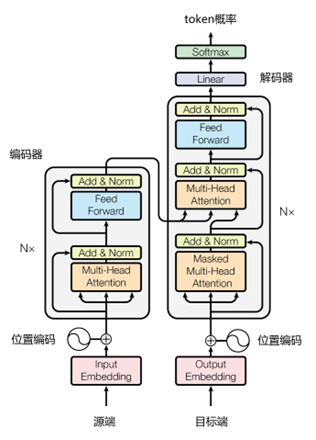
\includegraphics[width=1\textwidth]{figures/Transformer_Structure.png}
	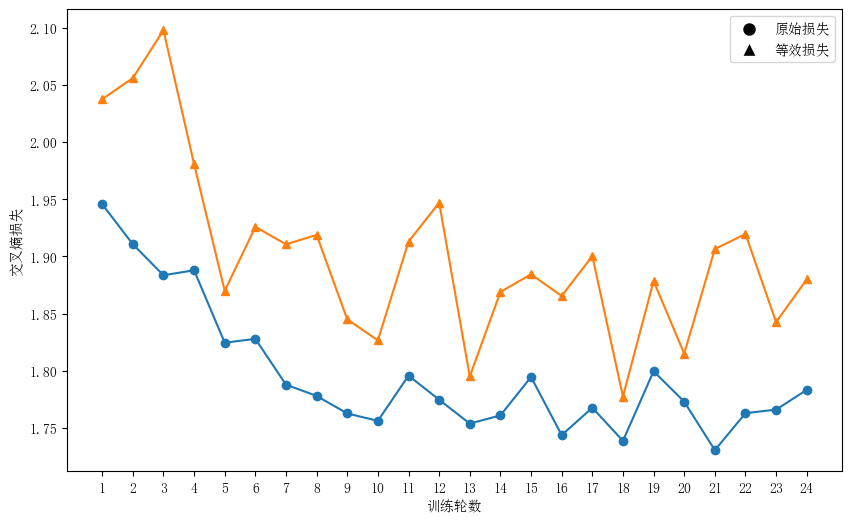
\includegraphics[width=0.8\linewidth]{figures/Chap4_clip_param_Loss.png}
	\caption{等效模型与原模型的训练损失对比}
	\label{Chap4_clip_param_Loss}
\end{figure}



%\begin{table}[]
%	\centering
%	\caption{等效模型与原模型的困惑度}
%	\begin{tabular}{|c|c|}
%		\hline
%		方式&困惑度
%		\\ \hline
%		原模型&$7.06$    \\ \hline
%		等效模型&$13.51$   \\ \hline
%		
%	\end{tabular}
%	\label{PPLComp}
%\end{table}

这种性能下降主要是由于模型权重量化以及函数近似导致的精度损失。不过值得注意的是,如果选择更高位数的量化情况,模型的表现效果应该会有所提升。总的来说,尽管等效模型在性能上略有下降,但在保护隐私的前提下,其仍然具有一定的应用价值。

%\subsection{实验分析}
(2)协议的开销分析与实验

表 \ref{communication_cost} 展示了 \ref{trans_block} 节中构建的Transformer模块的通信开销。其中$n$为输入矩阵的维度,这里的设定跟实际模型执行过程的设定相同,即每个矩阵为$n$维方阵;$l$为数据类型的比特数,如$l_{\text{float}}=32, l_{\text{int}}=32$;$p$为执行比较协议的小整数域$Z_p$的大小(本实验中$p=67$)。

\begin{table}[]
	\centering
	\caption{Transformer模块的通信开销}
	\begin{tabular}{|c|c|}
		\hline
		协议&通信开销
		\\ \hline
		Linear&$5n^2l$    \\ \hline
		Attention&$(30+5ks)n^2l+(8l\log(p)+24l)s$   \\ \hline
		FFN&$10n^2l+8l\log(p)+24l$   \\ \hline
		
	\end{tabular}
	\label{communication_cost}
\end{table}


表 \ref{Outsource} 展示了使用可验证外包计算的加速效果与输入维度的关系。其中,执行时间为所有在SGX上完成矩阵乘法的时间;传输时间为将数据从Enclave通过总线传到GPU以及计算结果从GPU通过总线传输回Enclave的总时间开销;验证时间为在Enclave中验证乘法结果计算正确性的时间;总外包时间包括了传输时间验证时间以及在GPU上的计算时间;加速比为执行时间与总外包时间的比值,反应了外包计算协议的执行加速效果。

\begin{table}[]
\centering
\caption{使用可验证外包计算的加速效果与输入维度的关系}
\begin{tabular}{|c|c|c|c|c|c|}
	\hline
	维度&执行时间&传输时间&验证时间&总外包时间&加速比
	   \\ \hline
	64&0.0001&0.0014&0.0002&0.0016&0.0753    \\ \hline
	128&0.0002&0.0016&0.0005&0.0011&0.1909    \\ \hline
	256&0.0021&0.0023&0.0012&0.0036&0.5930    \\ \hline
	512&0.0094&0.0072&0.0024&0.0098&0.9634    \\ \hline
	768&0.0257&0.0136&0.0041&0.0179&1.4419   \\ \hline
	1024&0.0611&0.0114&0.0085&0.0201&3.0509    \\ \hline
	2048&0.4173&0.0517&0.0486&0.1006&4.1497    \\ \hline
\end{tabular}
\label{Outsource}
\end{table}

可以看出,在矩阵计算维度为512时,二者计算开销大致相同,若维度小于512,则不使用外包计算的效果更好。反之,若维度大于512,使用外包计算的时间开销回更少,并且随着维度的增加,这个结果在不断扩大,在2048维时,通过外包计算的时间仅不到执行时间的1/4。

\section{本章小结}

%本章主要研究了在医学文本生成任务训练阶段中的隐私保护问题。首先,本章明确了系统模型和威胁模型,并设计了安全目标。随后,本章提出了基于秘密共享的多方计算协议来保障数据机密性,并使用Intel SGX保证执行过程的完整性。本章扩展了基于秘密共享的协议,使得可以构建复杂的Transformer结构。接着本章分析了协议的安全性,证明了协议满足设计目标。最后,本章通过实验验证了协议的有效性和高效性。

本章针对医学文本生成任务训练阶段的隐私问题,设计并实现了一种有效抵抗恶意攻击者的安全协议。本部分详细描述了系统模型、威胁模型以及安全目标,并扩展了基于加法秘密共享的协议来保护医疗数据的机密性,使之可以支持Transformer的复杂结构。此外,本章引入了SGX以确保医学文本训练协议执行的完整性,并设计了高效的外包计算协议以提高矩阵乘法的计算效率。最后,本章通过理论分析与实验验证,成功地验证了所提协议的安全性及高效性。